\documentclass{standalone}

\usepackage{tikz}
\usetikzlibrary{positioning, calc, arrows.meta, chains}

% new command: interval
\newcommand{\itv}[4]{ % #1: start point; #2: end point; #3: operation name; #4: style
  \coordinate (start #3) at #1;	% start point
  \coordinate (end #3) at #2;	% end point

  \draw[#4, |-|] (start #3) -- (end #3) % draw the interval
    node[pos = 0.5, above = 1mm,font = \Large, text=black] (#3) {$#3$}; % attach the operation name
}

\begin{document}
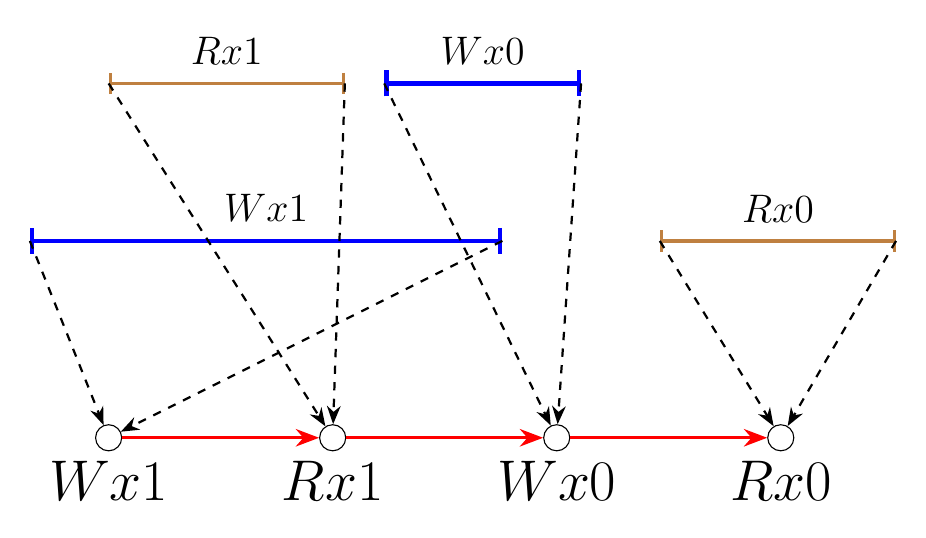
\begin{tikzpicture}[]

  \itv{(0,0)}{(6,0)}{Wx1}{ultra thick, blue};
  \itv{(8,0)}{(11,0)}{Rx0}{very thick, brown};

  % \itv{(1,2)}{(3,2)}{Wx0}{ultra thick, blue};
  \itv{(1,2)}{(4,2)}{Rx1}{very thick, brown};
  \itv{(4.5,2)}{(7,2)}{Wx0}{ultra thick, blue};

% atomicity schedule
\begin{scope}[font = \huge, start chain = atomicity, xshift = 1.0cm, yshift = -2.5cm, node distance = 2.5cm, every join/.style = {>=Stealth, very thick, ->, red}]
  \foreach \opi in {Wx1, Rx1, Wx0, Rx0}
    \node (\opi) [circle, draw, on chain, join, label = {[below] -90 : $\opi$}] {};
\end{scope}

% show the meaning of "atomicity"
\begin{scope}[atomicedge/.style = {>=Stealth, ->, dashed, draw, thick}]
  \foreach \opi in {Rx1, Wx0, Wx1, Rx0}{
	\draw[atomicedge] (start \opi) to (\opi);
	\draw[atomicedge] (end \opi) to (\opi);
  }
\end{scope}
\end{tikzpicture}
\end{document}